%% Creator: Inkscape inkscape 0.92.2, www.inkscape.org
%% PDF/EPS/PS + LaTeX output extension by Johan Engelen, 2010
%% Accompanies image file 'expb.eps' (pdf, eps, ps)
%%
%% To include the image in your LaTeX document, write
%%   \input{<filename>.pdf_tex}
%%  instead of
%%   \includegraphics{<filename>.pdf}
%% To scale the image, write
%%   \def\svgwidth{<desired width>}
%%   \input{<filename>.pdf_tex}
%%  instead of
%%   \includegraphics[width=<desired width>]{<filename>.pdf}
%%
%% Images with a different path to the parent latex file can
%% be accessed with the `import' package (which may need to be
%% installed) using
%%   \usepackage{import}
%% in the preamble, and then including the image with
%%   \import{<path to file>}{<filename>.pdf_tex}
%% Alternatively, one can specify
%%   \graphicspath{{<path to file>/}}
%% 
%% For more information, please see info/svg-inkscape on CTAN:
%%   http://tug.ctan.org/tex-archive/info/svg-inkscape
%%
\begingroup%
  \makeatletter%
  \providecommand\color[2][]{%
    \errmessage{(Inkscape) Color is used for the text in Inkscape, but the package 'color.sty' is not loaded}%
    \renewcommand\color[2][]{}%
  }%
  \providecommand\transparent[1]{%
    \errmessage{(Inkscape) Transparency is used (non-zero) for the text in Inkscape, but the package 'transparent.sty' is not loaded}%
    \renewcommand\transparent[1]{}%
  }%
  \providecommand\rotatebox[2]{#2}%
  \ifx\svgwidth\undefined%
    \setlength{\unitlength}{717.99998205bp}%
    \ifx\svgscale\undefined%
      \relax%
    \else%
      \setlength{\unitlength}{\unitlength * \real{\svgscale}}%
    \fi%
  \else%
    \setlength{\unitlength}{\svgwidth}%
  \fi%
  \global\let\svgwidth\undefined%
  \global\let\svgscale\undefined%
  \makeatother%
  \begin{picture}(1,0.80033404)%
    \put(0,0){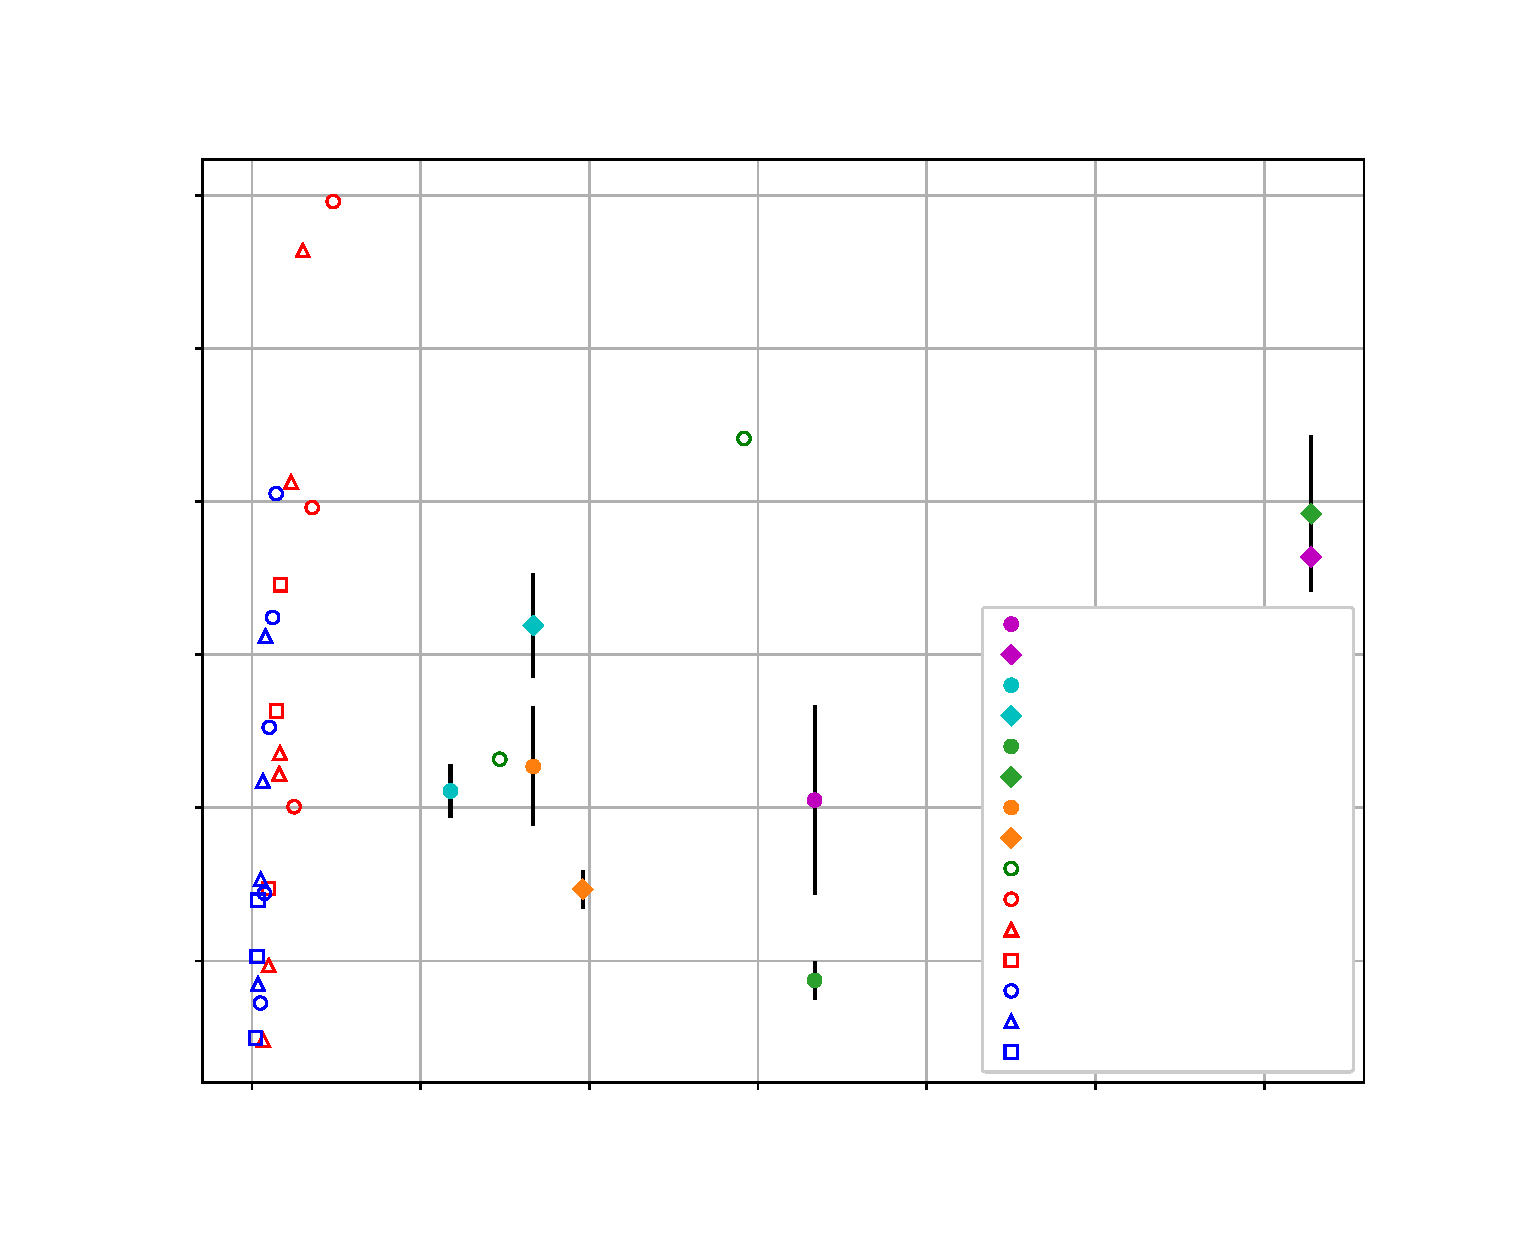
\includegraphics[width=\unitlength]{images_2ddl/expb.eps}}%
    \put(0.134617549,0.056780884){\color[rgb]{0,0,0}\makebox(0,0)[lb]{\smash{0.0}}}%
    \put(0.245897075,0.056780884){\color[rgb]{0,0,0}\makebox(0,0)[lb]{\smash{0.1}}}%
    \put(0.367176602,0.056780884){\color[rgb]{0,0,0}\makebox(0,0)[lb]{\smash{0.2}}}%
    \put(0.478455989,0.056780884){\color[rgb]{0,0,0}\makebox(0,0)[lb]{\smash{0.3}}}%
    \put(0.589735515,0.056780884){\color[rgb]{0,0,0}\makebox(0,0)[lb]{\smash{0.4}}}%
    \put(0.701015042,0.056780884){\color[rgb]{0,0,0}\makebox(0,0)[lb]{\smash{0.5}}}%
    \put(0.812294429,0.056780884){\color[rgb]{0,0,0}\makebox(0,0)[lb]{\smash{0.6}}}%
    \put(0.048357145,0.16405549){\color[rgb]{0,0,0}\makebox(0,0)[lb]{\smash{0.02}}}%
    \put(0.048357145,0.26643293){\color[rgb]{0,0,0}\makebox(0,0)[lb]{\smash{0.04}}}%
    \put(0.048357145,0.36881037){\color[rgb]{0,0,0}\makebox(0,0)[lb]{\smash{0.06}}}%
    \put(0.048357145,0.47118781){\color[rgb]{0,0,0}\makebox(0,0)[lb]{\smash{0.08}}}%
    \put(0.048357145,0.57356385){\color[rgb]{0,0,0}\makebox(0,0)[lb]{\smash{0.10}}}%
    \put(0.048357145,0.67594129){\color[rgb]{0,0,0}\makebox(0,0)[lb]{\smash{0.12}}}%
    \put(0.03510613,0.36174491){\color[rgb]{0,0,0}\rotatebox{90}{\makebox(0,0)[lb]{\smash{$H_{max} (m)$}}}}%
    \put(0.458455989,0.01){\color[rgb]{0,0,0}\makebox(0,0)[lb]{\smash{$F (N)$}}}%
    \put(0.678994986,0.38964463){\color[rgb]{0,0,0}\makebox(0,0)[lb]{\smash{\tiny PLA (50,5,2,34g)}}}%
    \put(0.678994986,0.36921009){\color[rgb]{0,0,0}\makebox(0,0)[lb]{\smash{\tiny PLA (50,5,2,64g)}}}%
    \put(0.678994986,0.34877694){\color[rgb]{0,0,0}\makebox(0,0)[lb]{\smash{\tiny PLA (60,5,1,12g)}}}%
    \put(0.678994986,0.3283424){\color[rgb]{0,0,0}\makebox(0,0)[lb]{\smash{\tiny PLA (60,5,1,17g)}}}%
    \put(0.678994986,0.30790786){\color[rgb]{0,0,0}\makebox(0,0)[lb]{\smash{\tiny PLA (50,4,2,34g)}}}%
    \put(0.678994986,0.28747332){\color[rgb]{0,0,0}\makebox(0,0)[lb]{\smash{\tiny PLA (50,4,2,64g)}}}%
    \put(0.678994986,0.26703878){\color[rgb]{0,0,0}\makebox(0,0)[lb]{\smash{\tiny PLA (60,8,1,17g)}}}%
    \put(0.678994986,0.24660424){\color[rgb]{0,0,0}\makebox(0,0)[lb]{\smash{\tiny PLA (60,8,1,20g)}}}%
    \put(0.678994986,0.2261697){\color[rgb]{0,0,0}\makebox(0,0)[lb]{\smash{\tiny Y&K acier(120,30)}}}%
    \put(0.678994986,0.20573516){\color[rgb]{0,0,0}\makebox(0,0)[lb]{\smash{\tiny Y&K polyimide(125,10)}}}%
    \put(0.678994986,0.18530062){\color[rgb]{0,0,0}\makebox(0,0)[lb]{\smash{\tiny Y&K polyimide(125,15)}}}%
    \put(0.678994986,0.16486608){\color[rgb]{0,0,0}\makebox(0,0)[lb]{\smash{\tiny Y&K polyimide(125,20)}}}%
    \put(0.678994986,0.14443293){\color[rgb]{0,0,0}\makebox(0,0)[lb]{\smash{\tiny Y&K polyimide(75,10)}}}%
    \put(0.678994986,0.12399783){\color[rgb]{0,0,0}\makebox(0,0)[lb]{\smash{\tiny Y&K polyimide(75,15)}}}%
    \put(0.678994986,0.10356357){\color[rgb]{0,0,0}\makebox(0,0)[lb]{\smash{\tiny Y&K polyimide(75,25)}}}%
  \end{picture}%
\endgroup%
